\documentclass{llncs}

\usepackage[a4paper,includeheadfoot,top=1.65in,bottom=1.65in,left=1.73in,hcentering]{geometry}
\usepackage[pdftex]{graphicx}

% Ezek egyikének bekapcsolásával a magyar ékezetes karakterek
% közvetlenül is felhasználhatók:
%\usepackage[latin2]{inputenc}
\usepackage[utf8]{inputenc}
%\usepackage{t1enc}


\usepackage{lmodern}
\usepackage[T1]{fontenc}


\usepackage{tikz-dependency}
\usepackage{qtree} % emmegmi? XXX
\usepackage{rotfloat} % \usepackage{float} helyett a sidewaysfigure miatt!
\restylefloat{figure}
\usepackage{tikz-qtree}

\usepackage{comment}

\usepackage[hungarian]{babel}
\selectlanguage{hungarian}

% saját cucc

\usepackage{amsmath}
\usepackage{graphicx}
\usepackage{wrapfig}
\usepackage{lscape}
\usepackage{rotating}
\usepackage{epstopdf}
\usepackage{hyperref}

%\usepackage{fullpage} % XXX ezt majd kukázni
%\parindent=0pt        % XXX ezt majd kukázni
%\parskip=6pt          % XXX ezt majd kukázni

\newcommand{\nyil}{$\rightarrow$\ }
\newcommand{\matnyil}{\ensuremath{\rightarrow}}
\newcommand{\nnyil}{$\leftrightarrow$\ }
\newcommand{\vnyil}{$\leftarrow$\ }
\newcommand{\code}[1]{\texttt{\small #1}}
\newcommand{\co}[1]{\texttt{\small #1}}
\newcommand{\embf}[1]{\textbf{#1}}
\newcommand{\bd}[1]{\textbf{#1}}
\newcommand{\cc}[1]{\multicolumn{1}{c}{#1}}

\renewcommand{\path}[1]{\code{#1}}
\DeclareMathOperator{\distop}{dist}
\newcommand{\dist}[2]{\ensuremath{\distop(\path{#1},\path{#2})}}
%{\sc dist}(\path{#1},\path{#2})}

\newcommand{\liex}[1]{\emph{#1}}

\newcommand{\ittt}{\fbox{\textbf{\_ITT\_T}}\ }

\definecolor{megjcolor}{rgb}{0.50,0.38,0.22} % -- kicsit sötétebb, jobban látszik
\definecolor{alertcolor}{rgb}{1.00,0.40,0.00} % -- durvább ;)
\definecolor{marcicolor}{rgb}{0.20,0.20,1.00} % -- durvább ;)
\newcommand{\XXX}[1]{{\small \color{megjcolor} [XXX #1]}}
\newcommand{\XXXb}[1]{\XXX{\embf{#1}}}
\newcommand{\XXXk}{\XXX{?}\ }
\newcommand{\XXXf}{\XXX{!}\ }
\newcommand{\XXXX}[1]{{\small \color{alertcolor} \bf [XXX #1]}}
\newcommand{\alert}[1]{{\color{alertcolor} \bf #1}}
\newcommand{\marci}[1]{{\color{marcicolor} #1}}

\newcommand{\hmsz}{$\blacktriangleright$} % egy háromszög
\newcommand{\para}[1]{\vspace*{6pt}\hmsz\ \embf{#1}\\}
\newcommand{\cpara}[1]{\vspace*{3pt}{\color{megjcolor}\hmsz\ #1}\\}

\newcommand{\sm}[1]{{\small #1}}
\newcommand{\smp}[1]{{\small (#1)}}
\newcommand{\kov}{\ensuremath{\implies}\ }
\newcommand{\azonos}{\ensuremath{\equiv}\ }
\newcommand{\kb}{\ensuremath{\sim}\ }
\newcommand{\term}[1]{\embf{#1}}

\newcommand{\degree}{degree} % XXX majd más lesz! :)
\newcommand{\bness}{bness}   % XXX majd más lesz! :)

\begin{document}

%\pagestyle{myheadings}
%\def\leftmark{{\rm XIV. Magyar Sz\'am\'\i t\'og\'epes Nyelv\'eszeti Konferencia}}
%\def\rightmark{{\rm Szeged, 2018. január 18-19.}}

%\setcounter{page}{1}

\title{A szöveg mint skálafüggetlen hálózat}
%a november 21-ig bekuldott verziobol kerjuk a szerzok adatait kihagyni
\author{Makrai Márton és Sass Bálint\\
  \institute{MTA Nyelvtudományi Intézet\break {\tt \{makrai.marton,sass.balint\}@nytud.mta.hu}}
}
\maketitle

% --------------------------------------------------------------------------

\begin{abstract}
Cikkünkben a szöveget egy egyszerű konstrukció segítségével
skálafüggetlen hálózatként ábrázoljuk,
és megvizsgáljuk, hogy a hálózatelmélet sztenderd eszközei
mit mondanak az ilyen módon reprezentált szövegről.
\\{\bf Kulcsszavak:} hálózatok, skálafüggetlen hálózatok, köztiség, Zipf, gyakoriság, szöveg
\end{abstract}

% --------------------------------------------------------------------------

\section{Bevezetés}
\label{sec:otlet}
% Sztem főként \cite{kovacs2012magyar} alapján...

% Def: sk-f h
Azokat a hálózatokat, ahol a befokszámok
Zipf-eloszlást követnek, \emph{skálafüggetlen hálózat}oknak nevezzük
\cite{barabasi1999emergence}
\cite[703.\ oldal]{kovacs2012magyar}.
%
Régóta tudjuk \cite{Zipf:1935}, hogy a szöveg szavainak gyakorisági eloszlása
Zipf-eloszlású.
% mi is a jó/sztenderd hivatk itt? done
%
Tanulmányunkban azt az élsúlyozott irányított gráfot vizsgáljuk, melynek
csúcsai a szóalakok, a $\langle w_1, w_2\rangle$ él súlya pedig a $w_1w_2$
bigram gyakorisága. Az előbbiek miatt ez a gráf skálafüggetlen.

Ebben a bevezető szakaszban
egy játékpéldán szemléltetjük a konstrukciót,
majd bemutatjuk a kapcsolódó irodalmat
és a HITS linkelemzési algoritmust,
amivel a leglátványosabb eredményeket kaptuk.
A következő szakaszban mutatjuk be a kísérleti eredményeket.

\subsection{Gráf bigramokból}
\label{sec:graph}

Az a feladat, hogy találjunk egy konstrukciót,
melynek segítségével a szövegbeli szógyakoriság
éppen a befokszám lesz egy alkalmasan megalkotott gráfban.
%
Így skálafüggetlen hálózatot kapunk.

% a konstrukció
Az ötlet nagyon egyszerű:
a hálózat csomópontjai a korpusz szavai lesznek,
menjünk végig a korpuszon és
minden szó esetén rajzoljunk be egy (1 súlyú) nyilat a hálózatba,
ami az adott szóból indul ki és őt közvetlenül követő szóhoz vezet.
%
Ha egy szópár többedszerre fordul akkor rajzoljunk be még egy nyilat,
vagy ami ezzel ekvivalens, a nyíl súlyához adjunk hozzá 1-et.
%
\Aref{fig:scfr_pelda}.\ ábrán látható hálózatot kapjuk.
%
Ez egy olyan gráf lesz, melyben a csomópontok szavak,
és az $A\matnyil B$ él akkor létezik, ha van $AB$ bigram a korpuszban,
és az él súlya $AB$ bigram gyakorisága.

\begin{figure}[ht]
\begin{center}
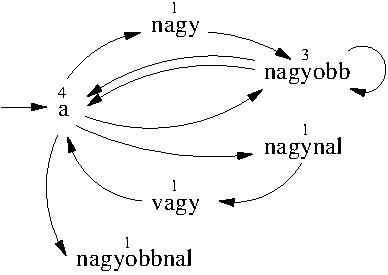
\includegraphics[width=6cm]{scfr_pelda.pdf}
\end{center}
\caption{,,A nagyobb nagyobb a nagynál vagy a nagy nagyobb a nagyobbnál.''
példamondat ábrázolása.
A dupla nyilat ábrázolhatjuk egy 2-es súllyal bíró szimpla nyíllal is.}
\label{fig:scfr_pelda}
\end{figure}

A fenti reprezentáció tehát skálafüggetlen hálózatot eredményez.
%
Ez azért nagyon jó, mert a skálafüggetlen hálózatok elméletének
% XXX egyrészt kamu, mert nem olvastam,
%     és nem is tudom mennyire jó kiindulópontnak,
%     másrész jó, mert sok fontos hivatkozás van benne! (+ rövid)
az elmúlt évek során kidolgozott összes
eszközét, módszerét, mérőszámát
\cite{barabasi2009scalefree}
% Marci: pár szóval hátrébb raktam a hivatkozást, mert ez a hivatkozás így, az
% "elmúlt évek" ürügyén kontrasztban van barabasi1999emergence-szel
alkalmazni tudjuk rá.

% "vmi értelmeset fog mondani"
Bízunk benne, hogy ezzel az eszköztárral
valami újat tudunk mondani a szövegről,
új módon tudjuk megragadni a szöveg bizonyos jellegzetességeit.

\subsection{Kapcsolódó irodalom}

% - vö: Varjú Zoli: "Kisvilágunk a nyelv"
%   itt (Ferrer és Solé, 2001) eljárását csinálja,
%   ami  \emph{nem pont az}, amit én írok! \XXXb{Ez nagyon kell!}
%   \nyil úh esetleg mégis érdekes lehet
%      egy MSZNY poszter erejéig megmutatni a gondolatomat! (!) XXX :)
%   -- de jó lenne, ha pont az enyémből jönnének olyan szép dolgok,
%      ami a Varjú Zoliéból nem, és pont azért, mert
%      nem csak a közvetlen rákövetkezést vette! (!) XXX :)

A mienkhez leghasonlóbb kutatás alighanem a TextRank \cite{mihalcea2004textrank}.
Mihalcea és Tarau az irányított, 2-széles ablakkal végzett kutatásaikról azt
írják, hogy rosszabb eredményeket hoztak, mint a az irányítatlan eset. Azt a
meglepő következtetést vonják le, hogy a szövegnek nincs természetes iránya.
Ha nyelvi adatból készült skálafüggetlen gráfról beszélünk, nem kerülhető meg
\cite{steyvers2005large} sem, ők azonban szemantikus hálókat vizsgálnak, míg mi
magából a korpuszból vonunk le első sorban szintaktikai tanulságokat.

% Fontos megjegyezni, hogy a fenti
A mi konstrukciónk lényegesen eltér attól a bevett megközelítéstől,
mely esetében akkor húzunk be egy (irányítatlan!) élt
két szó között, ha egy közös trigramban megtalálhatók,
más szóval, ha az egyik a másiktól (jobbra vagy balra)
1 vagy 2 szó távolságra van
\cite{cancho2001thesmall}.
Ennél a modellnél a szöveg természetes balról jobbra rákövetkezése
nincs reprezentálva,
szemben a mi modellünkkel, ahol viszont lényegi elem.
%
% XXX vö: szemantika vs. szintaxis!
Emiatt a most bemutatott modell várhatóan kevésbé szemantikai,
inkább szintaktikai jellemzőket tud majd megragadni.
%
% reviewer:
% "Milyen alkalmazásait tervezi a szerző a javasolt hálózatnak?"
% - mittomén, majd meglátjuk, alapkutatás! :)
A kutatás feltáró alapkutatás jellegéből adódóan
az eredmények esetleges majdani alkalmazása nem témája jelen cikknek.

A következő alszakaszban bemutatandó HITS algoritmus, amivel a leglátványosabb
eredményeket kaptuk.  nagyjából egyidős a skálafüggetlen gráfok ma népszerű
fogalmával.  Az utóbbi évtizedekben természetesen számos kutatás vizsgált
skálafüggetlen gráfokat a HITS segítségével \cite{zhang2007expertise}.

\subsection{HITS}

A HITS (Hyperlinkindukált témakeresés, \emph{Hyperlink-Induced Topic Search}
vagy hubok és tekintélyek, \emph{hubs and authorities}) egy linkelemzési
algoritmus \cite{Kleinberg:1999},
körülbelül egyidős a PageRankkel \cite{page1999pagerank}, csak persze sokkal
kevésbé elterjedt.
Az az alapötlete, hogy a fontos internetes oldalak kétfélék.  A \emph{hubok},
mint az \href{https://index.hu/}{index.hu} vagy a
\href{https://vajdasag.lap.hu/}{vajdasag.lap.hu}, nagy linkgyűjteményként
működnek: a rajtuk magukon megjelenő információnak nincs tekintélye, viszont
más, hiteles oldalakra, a \emph{tekintélyekre} irányítják a felhasználókat. A
hubok és a tekintélyek definíciója kölcsönös: jó hub egy olyan oldal, amely sok
tekintélyes oldalra mutat, nagy tekintélyük pedig azoknak az oldalaknak van
ebben a modellben, melyekre számos jó hub mutat.

A hub- és tekintélyérték számítása iteríatíve történik.  Kezdetben a számokat
tetszés szerint választjuk (például minden oldalnak ugyanazt), majd minden
iterációban egy oldal mértékadósága a rá mutató oldalak hubértékének összege
lesz, a hubérték pedig a lap által mutatott oldalak tekintélyének összege.  Az
iterációk között a hub- illetve tekintélyértékek négyzetösszegét normalizáljuk.
% bizonyos jelentős csomópontokat keres a hálózatban. A \emph{hub}-ok sok
% mindenkivel állnak kapcsolatban, az \emph{authority}-k pedig megbízható
% hiteles információt tudnak adni.  % XXX miről?
Ezzel az algoritmussal kaptuk a leginkább szembeötlő eredményünket.

\section{Eredmények}
\label{sec:results}

Vizsgálatainkat\footnote{\url{https://github.com/makrai/TextBetweenness.git}}
az MNSZ2 \cite{oravecz2014hungarian} véletlenül választott 1000 illetve 10000
mondatán végeztük.
%
Az elemzéseinkhez a NetworkX python csomagot használtuk
\cite{hagberg2008exploring}.



\subsection{Erős összefüggőség}
Az első nagyon egyszerű kérdés, hogy erősen összefüggő-e a gráf,
azaz minden szóból elérhető-e irányított úton az összes többi szó.
Lényegében erősen összefüggő lesz a gráf,
esetleg a korpusz elején és végén lévő
hapax szavakból álló ,,farok'' fordulhat elő,
ami megbontja az erős összefüggőséget
(ld.\ \aref{fig:scfr_pelda}.\ ábrán a \emph{nagyobbnál} szót).
% de hát biztos minden korpusz \emph{A}-val és ponttal végződik. :)

\subsection{Kisvilág tulajdonság}

A kisvilág-szerkezet szemléltetésére idézzük Karinthy 1929-es
\href{http://www.irodalmijelen.hu/05242013-1547/karinthy-frigyes-lancszemek}{\emph{Láncszemek}
című novellájá}t:

\begin{quote}
  Tessék egy akármilyen meghatározható egyént kijelölni a Föld másfél milliárd
  lakója közül, bármelyik pontján a Földnek – [a társaság egyik tagja fogadást
  ajánlott], hogy legföljebb öt más egyénen keresztül, kik közül az egyik neki
  személyes ismerőse, kapcsolatot tud létesíteni az illetővel, csupa közvetlen
  – ismeretség – alapon
\end{quote}

A meglepően kis távolság, melyet úgy formalizálhatunk, hogy az $L$ átlagos
távolság csak logaritmikusan növekszik a csúcsok számában, nem a
skálafüggetlen gráfok sajátja: Erdős--Rényi-féle véletlen gráfoknál is fennáll
\cite{erdos1960evolution}, ha a élek beválasztását kontrolláló $p$ elég nagy
ahhoz, hogy az egész hálózat összekapcsolódjon. (Vegyük észre a definícióban,
hogy önmagában egy gráf kisvilág tulajdonságáról nem beszélhetünk, csak egy
olyan gráfsorozat esetében, ahol a csúcsszám végtelenhez tart.) A kisvilág-szerkezet jellemzésében az alacsony $C$
klaszterezési együtthatót is meg szokták követelni \cite{watts1998collective},
de ennek az irányított gráfokra való általánosítása nem tűnik triviálisnak,
ezért tanumányunkban  a legrövidebb utak hosszából számított statisztikákra
szorítkozunk.  A mi 7 K-csúcsú, 13 K-élű gráfunkban az átlagos távolság
$L=4.89$. Az aszimptotikus tulajdonságot a poszteren elemezzük, amit a projekt
repójában talál meg az olvasó.
% maximálisan 19, ami lényegesen több, mint a közösségi hálókra Karinthy által
% helyesen megsejtett 6, de ez a hálózat irányítottságának köszönhető, írta
% Bálint, de Marci nem ért egyet, mert a közösségi gráfok is irányítottak.

\subsection{Skálafüggetlenség}

A skálafüggetlen gráfok definiáló tulajdonsága, hogy a fokszámok
hatványeloszlást követnek \cite{barabasi1999emergence}. Ezt nálunk Zipf
törvénye miatt biztosítja az, hogy (az első és az utolsó szó kivételével) a be-
és a kiélek súlyösszege egyaránt megegyezik a szónak a korpuszban való
gyakoriságával.  Az elméletileg garantált tulajdonságot statisztikailag is
ellenőriztük.  A fokszámeloszlást exponenciális eloszlással összehasonlítva
133-as likelyhood-ratiót és $5.91\cdot 10^{-6}$-os szignifikanciaszintet
kaptunk. A Zipf-együttható 2.20-nak adódott, ami összhangban van azzal, hogy az
angolban 1.25 körülre teszik \cite{Kornai:2008}, a magyar pedig gazdagabb
morfológiájú, így a Zipf-együttható is magasabbnak várható.

\subsection{Távolságok}
  Egy másik gráfmérték is hasznosnak tűnik az együtt-előfordulási gráf
    elemzésében, a csúcsok különcsége (\emph{eccentricity}), vagyis
    az adott csúcsból az összes többi
    csúcsba vezető legrövidebb utak hosszának maximuma.
    Míg a többi vizsgálatot
    tízezer mondatos mintán végeztük, az ebben a pontban említetteket csak ezer
    mondatoson, mert az összes (rendezett) csúcspárra ki kell hozzá számolni a legrövidebb
    út hosszát, aminek nagy az időkomplexitása.
    A \emph{sugár} (a legkisebb különcség) nálunk 9,
    az \emph{átmérő} (a maximális különcség) 19.
    Szemléletesen \emph{közép}nek \emph{(center)}
    % külterület}nek? szélnek? \emph{(periphery)}
    hívják azokat a pontokat, amelyeknek a különcsége megegyezik a sugárral.
    %z átmérővel.
    Esetünkben egy ilyen csúcs van, a sok funkcióban használatos vessző (,) token.
    % Kiszámoltuk a periphery-t is: ['Megadható', 'two']
    % -> \embf{center} = vessző (!) -- ez tetszik vmiért... :)

% \subsection{...}  TODO
% \bness\ csúnya az ábra, de nem eléggé
% XXX XXX végsőbe

\subsection{Closeness centrality}

A közelségi központiság (\emph{closeness centrality}) mértéke (mely
az adott csomóponttól az összes többi csomópontba vezető
legrövidebb utak hosszának átlagaként adódik)
% XXX wikipedia alapján...
% XXX és akkor nagy a clo-centr, ha ez az érték kicsi????
egy érdekes jelenséget mutat
(2.~ábra).  %\ref{fig:closeness}
%
A szavak egységes eloszlásban helyezkednek el.
Az eloszlásból néhány olyan elem lóg ki, amely
,,nem illeszkedik a magyar szövegbe'':
ilyen az egyenlőségjel és egy HTML entity ({\tt \&verbar;}),
illetve két angol szó (a \liex{the} és az \liex{of}),
melyek előfordulnak a korpuszban.
%
% Ez egy fokszám vs closeness_centrality grafikon, ugye?
Ezeknek a tokeneknek tehát kisebb
a közelségi központiság értékük annál,
mint amit gyakoriságuk alapján várnánk.
%
A kilógó elemek pontos karakterizálásához további vizsgálat szükséges.
%
% XXX Tudjuk értelmezni valahogy azt a helyet, ahol ő van? -> végsőbe

\begin{sidewaysfigure}[h]
\begin{center}
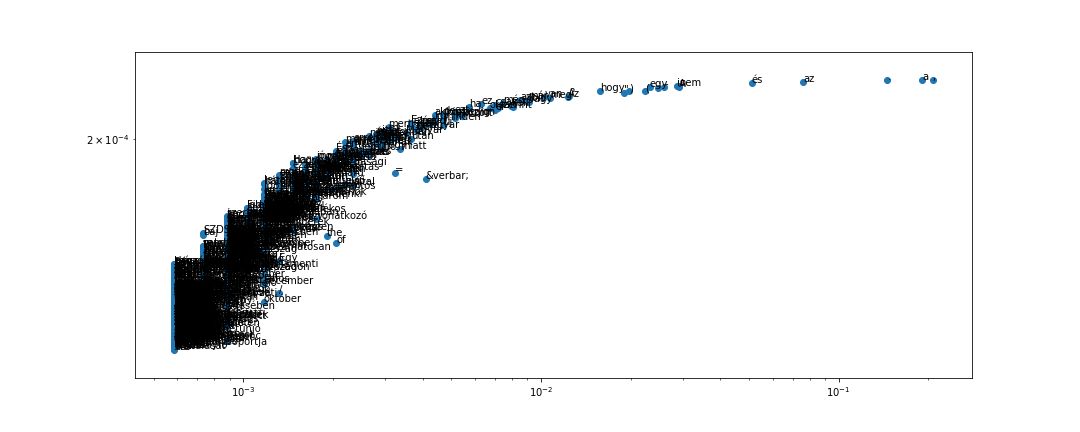
\includegraphics[width=25cm]{current-flow-closeness.png}
\caption{A szavak eloszlása \emph{closeness centrality} szerint.}
\end{center}
\label{fig:closeness}
\end{sidewaysfigure}

\subsection{HITS}

A bigramgyakorliságokból épített gráfban egy szó hubértéke az őt követő szavak
tekintélyének összege, egy szó tekintélyét pedig az őt megelőző szavak együttes
hubértéke adja.
%\Aref{fig:hits-auth}.\
A 3.~ábrán első körben azt látjuk, hogy a gyakoribb (nagyobb fokszámú)
szavaknak nagyobb a tekintélye -- ez nem meglepő. Érdekesebb, hogy a kötőszavak
és az igék jól elkülönülnek:
az egész szókincsre jellemző bal lent -- jobb fent átlótól inkább följebb vannak a kötőszavak,
és ettől az átlótól inkább lejjebb vannak az igék.
Azaz a kötőszavak tekintélye nagyobb annál, ami a gyakoriságuk alapján várható,
az igéké pedig kisebb.
% mit a szavaké általában.
% \embf{HITS / authorities} =
% bal-fent: kötőszavak, jobb-lent: igék\\
% \XXX{talán ez eddig a legérdekesebb, amit bele lehet magyarázni...}\\
% \liex{vagy} milyen szépen kilóg -- mert igének címkézzük (véletlenül),
% de a kötőszavak között van! (!) XXX :)
%
% reviewer kedvéért:
(Tehát nem egyszerűen arról van szó,
hogy a kötőszavak gyakorisága kiemelkedően magas,
hiszen az azonos gyakoriságú igék és kötőszavak is jól elválnak egymástól.)

% Az eredmény összefügghet azzal, hogy a kötőszavak
% lényegében mindenféle típusú elemmel kapcsolódni tudnak,
Az eredményre a következő intuitív magyarázatot javasoljuk: a kötőszavak nagy
tekintélye azt jelzi, hogy az őket megelőző tokenek együttes hubértéke nagy.
Mivel a szavak hubértéke az őket követő szavak tekintélyének összege, az ördögi
körből úgy léphetünk ki, ha a kötőszavak előtti tokenek után más tekintélyes
szavak is megjelennek. A gráf tehát tükrözi azt, hogy a kötőszavak olyan helyen
állnak, ahol a balkontextus alapján sok más szó is állhat. A tipikus példa
ilyen balkontextusra a már a center kapcsán is említett vessző token.
% az igék pedig -- ragaszkodva bővítményeikhez, vonzataikhoz --
% mindig ,,ugyanolyan'' elemekkel kapcsolódnak.
Az igék esetében épp ellenkező a helyzet: az igék előtt megjelenő szavak
(igemódosítók és bővitményi frázisok utolsó szavai) jobban determinálják, hogy
igének kell következnie, mint más szavak balkontextusa az adott szót.

\begin{sidewaysfigure}[h]
\begin{center}
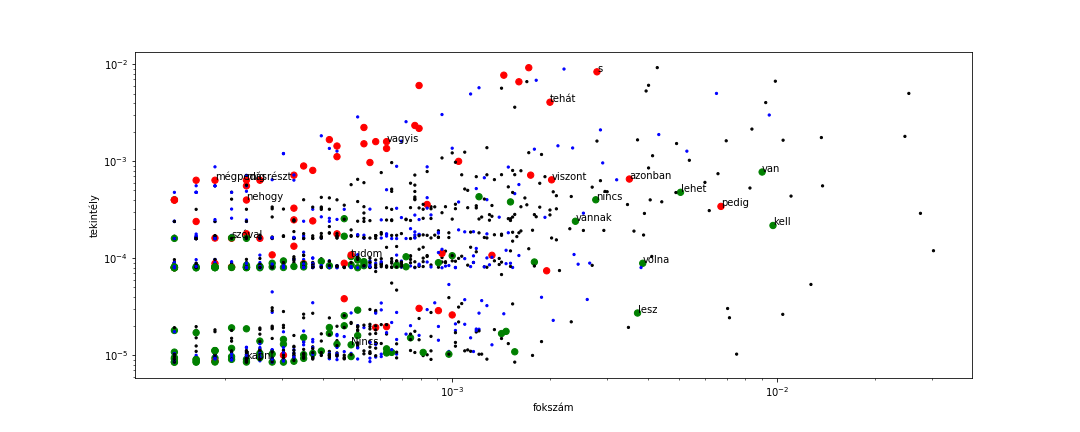
\includegraphics[width=25cm]{conv-verb-auth.png}
\caption{A HITS algoritmus eredménye.
A nagyobb piros ponttal jelölt kötőszavak balra fent
(magasabb authority),
a nagyobb zöld ponttal jelölt igék jobbra lent
(alacsonyabb authority)
helyezkednek el
a fokszám (gyakoriság) vs authority grafikonon.}
\end{center}
\label{fig:hits-auth}
\end{sidewaysfigure}


\section{Összefoglalás}

Az irányított skálafüggetlen hálózattá alakított szöveget
érintő első vizsgálatainkban feltérképeztük,
hogy az egyes hálózatelméleti eszközök
mit mondanak erről a hálózatról, milyen értékek a jellemzőek.
%
Legérdekesebb kezdeti eredményünk az,
hogy úgy tűnik, hogy a HITS algoritmus
képes egymástól elválasztani bizonyos szócsoportokat,
és ezek a csoportok összefüggésben vannak a szófajokkal.



\section*{Köszönetnyilvánítás}
\label{Koszonet}

Sass Bálint kutatásait
az MTA Bolyai János Kutatási Ösztöndíja támogatta
(ügyszám: BO/00064/17/1; időtartam: 2017-2020).


% ---- Bibliography ----
%
%kulon bibtex fajl hasznalata
\bibliographystyle{splncs}
\bibliography{minden.bib}

\end{document}
%\begin{comment}
% Marci: "Nem annyira zavarja, hogy egyedül csinálja,
%         de hát igen, a cikket meg kéne írni!"
% Marci: "Van olyan eset, hogy poszterre nem fogadják el?" :)
%
%   + cikk-kezdeményt csinálni -- megvan! :)
%
%   - cikk-kezdeménybe: az ötlet (pár hivatkozással!)
%     ! Marci: "írjam bele az ötletet, mert ha nem sok minden jön ki,
%               akkor a kontribúció jelentős része maga az ötlet lenne!" (!)
%
%   - cikk-kezdeményt közösen szerkeszthetővé tenni
%     ? github? overleaf? (?) XXX :)
%       -- asszem az utóbbi lesz, nincs jobb ötletem :)
%     ! Marci, ne törölj légyszi, semmit se! :)
%
%   - beletenni mindent, ami van :)
%     ! nézzem meg a Marci-féle megosztott doksit
%
%   - kitalálni a további teendőket :)
%
%   - megcsinálni a további teendőket :)
%
%   - beadás előtt: .tex: fullpage-t kukázni! :)

% \marci{Ha nem nagy teher, akkor légyszi így írj bele, Marci. :)}

% nyilván jó lenne 2 bevezető mondat a hálózatelméletről. -- kb oké.
% HIVATK: Barabási-Albert (eredeti cikk), -- vmit betettem...
%         Csermely (közérthető). -- sztem majd a végsőbe tegyük bele XXX

\section*{XXX Bírálatok XXX}

\subsection*{XXX Első bíráló XXX}

\begin{itemize}

\item[+]
"nagyon érdekes kísérleteket"
"jelentős tudományos eredmények is születhetnek a kísérletekből"
  -- köszi :)

\item[+]
"hiányzik az előzmények, az alternatív megoldások bemutatása"
  -- fogalmunk sincs... :)

\item[+]
"hiányzik az eredmények komparatív kiértékelése"
  -- há mer új az ötlet! :)

\item
"hiányzik azoknak a fogalmaknak a magyarázata,
amelyeket a cikkben minimális definiálás után használnak (pl. különcség )."
  - \embf{Marci, ez jó lenne!}

\item[+]
"igen rövid az összefoglalás"
  -- hm.. :)

\item
"igen rövid az irodalomjegyzék"
  - \embf{Marci tedd bele légyszi a hivatkozásaidat
(3 db) az irodalomjegyzékbe :)}
\embf{Zipf-re nem tudod esetleg a tuti hivatkozást
a \ref{sec:otlet}.\ rész elejetájára?}

\end{itemize}

\subsection*{XXX Második bíráló XXX}

\begin{itemize}

\item[+]
"Nem derül ki, hogy mi a célja a vizsgálódásnak azon túl, hogy 'Bízunk
benne, hogy ezzel az eszköztárral valami újat tudunk mondani a szövegről'."
  -- há mer ez a célja :)

\item[+]
"A dolgozat egyetlen következtetést sem von le."
  - nana! dehogynem!

\item[+]
"Milyen alkalmazásait tervezi a szerző a javasolt hálózatnak?"
  - mittomén, majd meglátjuk, alapkutatás! -- \emph{Ezt beleírtam.}

\item[+]
"A dolgozat stílusa nem éri el egy tudományos publikáció színvonalát (pl.
'Az ötlet nagyon egyszerű: menjünk végig a korpuszon és minden szó
esetén rajzoljunk be egy (1 súlyú) nyilat.'),"
  -- sztem ez teljesen oké így. :)

\item
"elfogadás esetén a szövegezés erős javítása szükséges."
  - esetleg lehetne tenni vmit ezzel... \embf{Esetleg... Hm? :)}

\item[+]
"A 2. fejezetben közölt számok mekkora és milyen korpuszból épített hálózat
jellemzői?
  - \emph{Ezt beírtam a \ref{sec:otlet}.\ rész végére. Jó így, nem? :)}

\item[+]
"Az, hogy a kötőszavakat elkülöníti a HITS nem egyszerűen annak köszönhető,
hogy azok gyakorisága kiemelkedően magas?"
  -- \emph{Ezt beleírtam.}

\end{itemize}

\subsection*{XXX Egyebek XXX}

\begin{itemize}

\item
\bness\ "csúnya az ábra, de nem eléggé" (alább)
-- \embf{ezzel van vmi? Be lehet tenni a végsőbe? :)}

\item[+]
closeness centrality grafikon:
Tudjuk esetleg értelmezni valahogy azt a helyet,
ahol ezek a kilógó izék vannak?
  -- \emph{Ezt beleírtam.}

\item
closeness centrality grafikon:
\embf{Esetleg bele tudsz nézni kicsit közelebbről ebbe az eloszlásba?
Mi van az alján, mi van a tetején?}

\item
  \embf{A két 9-es ugyanaz a dolog?} javítottam, mostmár csak egy 9-es van.
    (És két 19-es, ami ugyanaz, de az egyik kommentben.)

\item
\embf{Stimmel, hogy kerület == különcség=sugár? nem különcség=átmérő?
A vessző az egyetlen 9-es?}
    a sugár és az átmérő számok, a közép és a periphery halmaz
    sugár = min különcség
    átmérő = max különcség
    közép = {v: különcség(v) = sugár} = {,}
    igen, vessző az egyetlen
    periphery = {v: különcség(v) = átmérő}
    de erről nem írunk

\item
Nem jöttem rá, hogy ez miért nem működik:
\verb=\Aref{fig:hits-auth}=
\embf{Van tipped? :)}


\end{itemize}

\section{Friss ,,betweenness'' jegyzetek XXX}

Kérdés: tényleg arányos-e örökké (annak kell-e lennie),
a \degree\ és a \bness?\\
\embf{Mosmá kijött, hogy nem!}\\
= van olyan, hogy ,,\degree\ sok + \bness\ kevés''
(= ez mi is lenne ábrával?)\\
meg hogy ,,\degree\ kevés + \bness\ sok''
(= ugye ez az, hogy két gombolyag összekötve egy vonallal)\\
-- vagy legalább az egyik előfordul. :)

\embf{2017.11.23.\ A csúnya ábrát nagyon szeretem,
az eddig a főfő eredményünk! (!) XXX :)}\\
\XXXb{Sikerül annotálni?
Mely szavak vannak vajon az egyes kitüntetett pontokon?}

-----

 - Shahadat Uddin et al.:
Network Effects on Scientific Collaborations\\
%
,,\degree\ sok + \bness\ kevés'' esetről azt mondja hogy:
"It could be explained by the fact that some authors have high number of collaborations with many different other authors; however, they do not play a bridging role in the co-authorship network."

- Carlo Morselli:
Assessing Vulnerable and Strategic Positions in a Criminal Network\\
% [./morselli_highlow_10.1.1.1027.9852.pdf]
%
szép ábra (Figure 1): \degree\ vs \bness 4 variációja! (!) XXX :)
% Qin Wang is mondja, hogy van ilyen, csak csúnyább az ábrája... :)

\bness: el lehet mondani, amit ezekről szoktak:
\begin{itemize}
\item
central = ,,Most important actor'' (Ann McCranie diái szerint)
\item
high \bness\ = ,,cutpoint''
wikipedia: ,,Betweenness centrality is related to a network's connectivity, in so much as high betweenness vertices have the potential to disconnect graphs if removed.''
Ha kiszedjük a ,,\bness\ sok'' pontokat, akkor szétesik a hálózat.
Kérdésem: mire esik szét?
Marci szerint nem érdekes, mert folytonos lesz a szétesés...
\end{itemize}

-----

infó a dolgokról:
\code{https://networkx.github.io/documentation/networkx-1.10/reference/algorithms.html}

-----

ezt mondom:
Az összes mérték azért van, mert nem látjuk a gráfot,
és ezekkel szeretnénk látni. :)

%\end{comment}

% --------------------------------------------------------------------------

\end{document}

\section{Vizsgálandó dolgok XXX :)}

\begin{itemize}
\setlength\itemsep{1em}

\item
\embf{erős összefüggőség?}
Az lesz.

2017.11.21. \embf{Marci: erősen (=irányítottan) összefüggő-e a gráf? :)}
Válasz: \embf{hát igen!}
Az \ref{fig:scfr_pelda}.\ ábrán ugye a \emph{nagyobbnál} lóg ki egyedül,
szóval ilyen korpusz elején és végén lévő
különleges szavakból álló ,,farok'' lehet,
ami esetleg nem erősen összefüggő,
de hát biztos minden korpusz \emph{A}-val és ponttal végződik. :)

\item
ugye \embf{kisvilág} a gráfunk?\\
= minden mindenből elérhető mondjuk 6 lépésben
[= legrövidebb utak max hossza 6]\\
\XXXb{Mi a helyzet ezzel?}
%
Marci szerint 2 lesz vagy 3. :)
%
Eredmény:
radius = 9; \embf{diameter = 19 (!)} -- a Karinthy-féle 6 helyett
%
Def: mi a small-word-ség definíciója? (?) XXX :)
ld. https://en.wikipedia.org/wiki/Small-world\_network (!)
= hogy vmi logaritmikus + a clustering coeff ,,nagy''.

\item
\embf{centralitás?}

\begin{itemize}

\item
\emph{[lokális]} \embf{degree centrality} --
Ha ez magas, akkor
,,A csúcspont központi szerepű a lokális környezetében.''
\cite{kovacs2012magyar}.

Jó, ez trivi:
degree centrality \azonos szógyakoriság.
A gyakori szavak azok, amiknek nagy
a degree-centrality-je (befokszám-összege),
és tényleg ők bizonyos értelemben a legfontosabb szavak.

2017.11.21. \embf{Marci:}
,,10 k mondatot nézek.
Odaig jutottam, hogy valóban power law a degree centrality.''
Jó, akkor a kiindulópont megvan (= szöveg szavainak gyakorisága Zi pf). :)
Azaz ez kísérletileg is kijött.

\embf{Ez okés! :) Ez trivi, nem annyira eredmény,
inkább csak ellenőrzés, hogy jó volt-e a kiindulópontunk.}

A \embf{csúcserősség} (esetünkben) tök ugyanez: benyíl-súlyösszeg.

\item
\emph{[globális]} \embf{köztiség (betweenness)}.
Def: (\cite{kovacs2012magyar}-ban sztem zavaros)
sztem: hány legrövidebb út meg át a csomóponton;
avagy: a legrövidebb utak hány \%-a megy át a csomóponton.\\
\XXXb{Mi a helyzet ezzel?}\\
\XXXb{SEJTÉS: olyasmit vélek, hogy ez összefőgg vhogy a szófajokkal,
vagy legalábbis vmilyen típusú szavaknak nagyobb/kisebb lesz.
Pl.\ a névelőnek nem nagy? [Ez már egy bazi jó eredmény lenne sztem!]}

\item \embf{closeness centrality} is van -- de sztem most hagyjuk :)

\end{itemize}

\item
\embf{sűrűség?}
,,Ha egy hálózati csúcspont néhány lépéses környezetén belüli csúcspontok között viszonylag sok él van, akkor a hálózatnak ezt a tartományát sűrűnek mondjuk.''\\
\XXXb{Mit tudunk mondani a sűrűségről általában? Vagy sűrű tartományokról? Vannak? Hogy is lehet őket megtalálni?}

\item
\embf{$k$-mag?}
Def: $k$-mag = ,,azok a csúcspontok tartoznak ugyanahhoz a $k$-maghoz, amelyek legalább $k$ számú kapcsolattal kötődnek a magban lévő más csúcspontokhoz.''\\
\XXXb{Mit tudunk mondani a $k$-magokról? Hogy találjuk meg őket?}

\item
\embf{csoportok? (=klikkek?)}
Asszem annyi, hogy belül sűrűek. Csoportszerkezet? (átfedések...)\\
\XXXb{Mit tudunk mondani a csoportokról?
Van a kezünkben csoportkeresési eljárás?
Pl.\ klikk perkolációs algoritmus? (ami magyar találmány elvben)
Átfedhetnek!}

\item
nemcsak \emph{centrality} van, hanem \emph{prestige} is:
a legfontosabb prestige index: \embf{rank} (Ann McCranie diái)

\end{itemize}

\section{Korábbi jegyzetek XXX}

\code{https://github.com/makrai/TextBetweenness} \XXXf

 * ötlet: ,,a szöveg skálafüggetlen hálózat'' -- mondjuk elég trivi ötlet! :)
 -- alapötlet:
    \emph{azért Zipf a szavak, mert vhogyan skálafgtlen hálózatot alkot!}
    \smp{ugye, hogy NEM a szemantikai, szóasszoc, meg hasonló hálózatokkal
         szórakozunk mostan! :)}

 * http://www.greenteapress.com/compmod/html/book006.html
 * https://arxiv.org/pdf/cs/0701135 // 2.2.3 konkrétan :)
 * (Kornai sok Zipf-et ír a matnyelv könyvében, esetleg ezt is említi?)
 \nyil szóval úgy tűnik, hogy ezt már réges rég leírták.
    (azért erre lehetett számítani...)

 \embf{De:} ténylegesen kimondták azt, hogy
 \emph{így (simán közvetlen rákövetkezéssel)
 lehet megkonstruálni a hálózatot, aminek a befokszám összege
 éppen a szógyakoriság lesz, amiről meg (eleve, rég) tudjuk, hogy Zipf,
 azaz skálafüggetlen lesz ez a hálózat
 (éppen mivel a befokszáma Zipf)???} (?!) XXX :)

 -- az itt a nagy eredmény, hogy ez egy skálafüggetlen network lesz, azaz
    minden érvényes lesz rá, ami a skálafüggetlenekre érvényes! (!) XXX :)

 -- de hogy akkor az lenne az "új", hogy erre a hálózatkutatás
    minden eredménye akkor alkalmazható lesz! (!) XXX :)
    -- pl. a "növekedési mechanizmus"-t be lehet mutatni,
       miszerint jön egy új szó, az a növekedési tulajdonság szerint
       illeszkedik be, ez biztosítja, hogy megmarad a skálafüggetlenség! XXX

 \nyil ez nyilván egybecseng a nyelvmodellekkel,
    amik a szavak egymásra következéséről szólnak! (!) XXX :)

 -- szóval ez a két dolog (szavak Zipf \nnyil skálafüggetlen hálózatok)
    akkor oda-vissza szépen megmagyarázza egymást!

 - vö: Varjú Zoli: "Kisvilágunk a nyelv"
   itt (Ferrer és Solé, 2001) eljárását csinálja,
   ami  \emph{nem pont az}, amit én írok! \XXXb{Ez nagyon kell!}
   \nyil úh esetleg mégis érdekes lehet
      egy MSZNY poszter erejéig megmutatni a gondolatomat! (!) XXX :)
   -- de jó lenne, ha pont az enyémből jönnének olyan szép dolgok,
      ami a Varjú Zoliéból nem, és pont azért, mert
      nem csak a közvetlen rákövetkezést vette! (!) XXX :)

-----

az élsúlyok persze a bigramok, ez trivi.
\smp{az $n$-gramok ($n > 2$) viszont totál nem jelennek meg ebben!}

Viszont a hálózat csomópontjai nem ,,egyneműek'': szófajok vannak.
Ez különleges lehet a sima skálafüggetlen hálózatokhoz képest
(vö: emberek+kutyák hálózata).

A névelőnek sztem nagy lesz a \emph{köztiség (betweenness)} értéke,
és a szófajok talán kijönnek \emph{csoport}okként! :)
\smp{Varjú Zoli mit is ír a funkciószavakról? :)}

\embf{TÖK FONTOS:}
\path{a2a} (\dist{a}{a}=2) nem jelenti azt, hogy van \path{axa} trigram,
csak annyit jelent, hogy van \path{ax} és \path{xa} bigram!
\smp{ez benne az új, izgi! :) [ez is]
-- hm.. bár lehet, h pont ezt tudja
   100 éve trivi módon a sima bigram modell
   \nnyil azért a betweenness meg ezek, hogyzhatnak újat! (!) XXX :)
-- hogy mire lesz jó, azt persze még nem tudom. :)}

-----

Vannak határozott \emph{irányok}
(ti.\ ami csak egyik irányba hajlamos menni), pl.\ névelő \nyil fn.
Ez nem hat a skálafüggetlenség ellen? Talán nem. (Sztem nem.)

-----

Legrövidebb utak kiszámolása:
nem megy ez a régi concgram-es ,,mindent egyszerre, amit épp tudunk''
ötletem alapján? De sztem megy.
\embf{ld.\ a külön papírkát, ahol bemutatom! -- azt beírni!! :)}

Bár biztos van rá 100 más (jobb) módszer... :)

-----

Persze nem csak szavakra megy, hm lemmákra, POS-tagekre, morfémákra.
Hiszen (közismerten) mind Zipf. :) Ezeket is lehet nyomni.

-----

XXX Pollner Péter adna esetleg hozzá szoftvert,
ami alap dolgokat számolgat? :)

XXX többi (esetleg kapcsolódó) megjegyzés
\cite{kovacs2012magyar} kapcsán: {\tt mk.INFO}.

ilyenek:
-- "szerveződési mintázatok keresése" community detection\\
-- van-e hozzá szoftvercsomag, amivel alap mutatókat lehet számolni?\\
-- további irodalom hozzá

-----

shortest path: gondolkodtam rajta (papírka),
de persze van a Floyd-Warshall algó... :)

-----

toolkit: \embf{NetworKit}
linkgroup (Csermely Péter) / links / Network analysis
-- Get started + NetworKit User Guide, \emph{kipróbálni nagyon!}

2017.11.08. vagy esetleg épp Neo4j -vel lenne érdemes csinálni? :)
% https://db-engines.com/en/article/Graph+DBMS

2017.11.14. Vedres Balázs: "az elemzést Matlab-ban végeztem,
csak az alap mátrixaritmetikai funkciókkal. A NetworKit-et nem ismerem."
-- hú és akkor hogy számolt betweenness-t, meg klikk-perkolációt, stb-t? :)


-----

ACL Anthology: search: scale-free, NetworKit
\nyil foglalkozott ezzel bárki?\\
\embf{"scale-free" bigram} \nyil 20 találat, ezeket végig kell nézni! XXX :)\\
\embf{"scale-free" bigram betweenness} \nyil 3 találat, ezeket még inkább! XXX :)

-----

ez a scale-free bigramos modell tökre segíthet kitalálni a pázmányos
elemző dolgait! :) merthogy pont a rákövetkezési szabályokról mond vmit! :)

-----

persze a "2-vel utána következő szó"-ból is scale-free network jön ki
(lényegében tuti, de azért ellenőrizzem),
aminek első ránézésre nem sok teteje van, de ki tudja... :)

-----

CEU Center for Network Science -- Vedres Balázs, Kertész János

-----

azzal, hogy a sorrend nálam nagyon számít
(vö: \cite{kovacs2012magyar} simán szimmetrikus ablakot vett)
\emph{szemantikus} helyett \emph{szintaktikus} hálózatot kapunk
= reményem szerint kijönnek a szófajok.

-----

meetup Berend Gáborról:
,,he also has a keen interest in network science'' (!) :)
